\documentclass[../problems.tex]{subfiles}

\graphicspath{{../images/}}

\begin{document}
\section{Momentum and Angular Momentum}
\barh 

\paragraph{3.1}

The speed of the shell relative to the ground is defined as $v_s=v + v_g$  or $v_g = v_s - v$ where
$v_g$ is the speed of the gun relative to the ground. Using conservation of momentum
\begin{align*}
    P_i &= P_f \\
    0 &= mv_s + Mv_g \\
    0 &= mv_s + M(v_s - v) \\
    v_s(m + M) &= Mv \\
    v_s &= \frac{Mv}{m + M} \\
    v_s &= v \frac{1}{1 + m/M}
\end{align*}

\paragraph{3.3}

Let the mass of each fragment be $m$ and the mass of the shell be $3m$. The total momentum is
\begin{align*}
    3m\vb{v}_o &= m\vb{v}_1 + m\vb{v}_2 + m\vb{v}_3 \\
    2\vb{v}_o &= \vb{v}_2 + \vb{v}_3 \\
\end{align*}
since $\vb{v}_1 = \vb{v}_o$. Split into components
\begin{align*}
    2v_o &= v_2(\cos{\theta_2} + \cos{\theta_3}) \\
    0 &= v_2(\sin{\theta_2} + \sin{\theta_3}) = \sin{\theta_2} + \sin{\theta_3} \\
\end{align*}
where $v_2=v_3$. Since $\theta_2=\theta_3+\pi/2$
\begin{align*}
    \theta_3 = -(\pi/2 - \theta_2)
\end{align*}
and
\begin{align*}
    \cos(\theta_3) &= \cos(-(\pi/2 - \theta_2)) = \sin(\theta_2) \\
    \sin(\theta_3) &= \sin(-(\pi/2 - \theta_2)) = -\cos(\theta_2)
\end{align*}
in the second equation
\begin{align*}
    0 &= \sin{\theta_2} - \cos{\theta_2} \\
    \sin{\theta_2} &= \cos{\theta_2} \\
    \tan{\theta_2} &= 1 \\
    \theta_2 &= \pi/4
\end{align*}
and $\theta_3 = -(\pi/2 - \pi/4) = -\pi/4$. Substituting back into the first equation
\begin{align*}
    2v_o &= v_2 (\cos(\pi/4) + \cos(-\pi/4)) \\
    2v_o &= v_2 \frac{2}{\sqrt{2}} \\
    v_2 &= v_o\sqrt{2}
\end{align*}
% figure of the shell exploding into 3 pieces
\begin{figure}[ht]
    \centering
    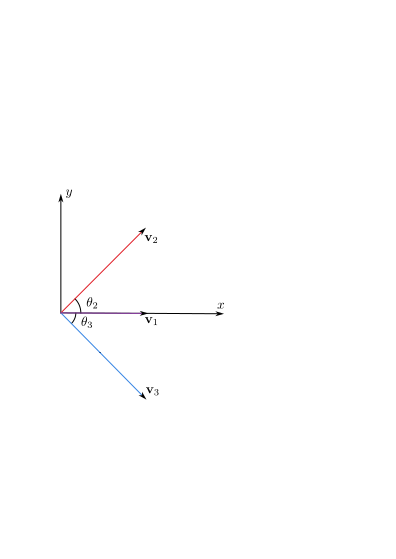
\includegraphics[width=0.3\linewidth]{../images/fig3_3.png}
    % caption width is 0.9\linewidth
    \captionsetup{width=0.7\linewidth}
    \caption{A shell exploding into three pieces. When $\vb{v}_1$ is solely in the positive
    $x$ direction, $\theta_2 = \pi/4$ and $\theta_3 = -\pi/4$.}
    \label{fig:3_3}
\end{figure}
The three velocities are sketched in Figure \ref{fig:3_3}.

\newpage
\paragraph{3.5}

In an elastic collision the bodies stay seperated after the collision. The conservation of momentum:
\begin{align*}
    P_i &= P_f \\
    m_1 \vb{v}_1 + m_2\vb{v}_2 &= m_1\vb{v}_1' + m_2\vb{v}_2'
\end{align*}
where $\vb{v}_2 = 0$ and $m_1 = m_2$ so the equation becomes
\begin{equation*}
    \vb{v}_1 = \vb{v}_1' + \vb{v}_2'
\end{equation*}
From the conservation of energy:
\begin{align*}
    E_i &= E_f \\
    \frac{1}{2}m_1v_1^2 &= \frac{1}{2}m_1v_1'^2 + \frac{1}{2}m_2v_2'^2 \\
    v_1^2 &= v_1'^2 + v_2'^2
\end{align*}
Squaring the first equation
\begin{align*}
    v_1^2 &= v_1'^2 + v_2'^2 + 2\vb{v}_1' \cdot \vb{v}_2' \\
    0 &= 2\vb{v}_1' \cdot \vb{v}_2' \\
    \vb{v}_1' \cdot \vb{v}_2' &= 0
\end{align*}
The dot product is zero when the vectors are perpendicular, therefore the angle between the two
vectors is $\pi/2$ or $\qty{90}{\degree}$ Q.E.D.

\paragraph{3.7}

The equation of the rocket's motion given by is
\begin{equation*} \tag{3.8}
    v - v_o = v_{ex} \ln{\frac{m_o}{m}}
\end{equation*}
Since $v_o = 0$ the velocity of the rocket is
\begin{align*}
    v &= v_{ex} \ln{\frac{m_o}{m}} \\
    &= \qty{3000}{\meter/\second} \ln{\frac{\qty{2e6}{\kilo\gram}}{\qty{1e6}{\kilo\gram}}} \\
    &= \qty{3000}{\meter/\second} \ln{2} \\
    v &= \qty{2100}{\meter/\second}
\end{align*}
solving for thrust
\begin{align*}
    \textrm{thrust} &= -\dot{m} v_{ex} \\
    &= - \frac{\dd{m}}{\dd{t}} v_{ex} \\
    &= -\frac{\qty{1e6}{\kilo\gram}}{\qty{120}{\s}} * \qty{3000}{\meter/\second} \\
    &= -\qty{-2.5e7}{\kilo\gram.\m/\second^2}
\end{align*}
where thrust is in newtons. In comparison, the thrust is larger than the initial weight:
\begin{align*}
    m_og= \qty{2e6}{\kilo\gram}*\qty{9.81}{\meter/\second^2} = \qty{1.96e7}{\kilo\gram.\m/\second^2}
\end{align*}

\paragraph{3.9} 

The equation $m_og = -\dot{m}v_{ex}$ describes when the magnitude of thrust equals the initial
weight. Solving for the minimum exhaust speed
\begin{align*}
    v_{ex} &= \frac{m_og}{-\dot{m}} \\
    &= \frac{\qty{2e6}{\kilo\gram}\cp\qty{9.81}{\meter/\second^2}\cp\qty{120}{\s}}
        {-\qty{1e6}{\kg}}\\
    &= -\qty{2350}{\meter/\second}
\end{align*}

\paragraph{3.11}
(a) The change in total momentum of the system is given by
\begin{equation*}
    \tag{3.4}
    \dd{P} = m \dd{v} + \dd{m} v_{ex}
\end{equation*}
Since there is a net external force, $\dd{P} = F^{ext} \dd{t}$. Dividing both sides by $\dd{t}$
\begin{align*}
    \frac{\dd{P}}{\dd{t}} &= m \dv{v}{t} + \dv{m}{t} v_{ex} \\
    F^{ext} &= m \dot{v} + \dot{m} v_{ex}
\end{align*}
hence, the equation of motion is
\begin{align*} \tag{3.29}
    m\dot{v} &= - \dot{m} v_{ex} + F^{ext}
\end{align*}
(b) In the Earth's gravitational field the external force is $F^{ext} = -mg$. Assuming a constant
ejected mass $\dot{m} = -k$, the mass of the rocket is $m = m_o - kt$ where $m_o$ is the initial
mass of the rocket. Substituting into the equation of motion
\begin{align*} \tag{3.30}
    m\dot{v} = -\dot{m} v_{ex} - mg
\end{align*}
separating variables and integrating
\begin{align*}
    \dot{v} &= \frac{k}{m} v_{ex} - g \\
    \dd{v} &= \quantity(\frac{kv_{ex}}{m_o-kt}-g) \dd{t} \\
    \int_{v_o}^{v} &= \int_{0}^{t} \frac{k}{m_o-kt} \dd{t} - \int_{0}^{t} g \dd{t} 
\end{align*}
Using u-sub: $u = m_o - kt$ and $\dd{u} = -k \dd{t}$, where $u(0) = m_o$, $u(t) = m_o - kt = m$, and
$v_o = 0$
\begin{align*}
    v - v_o &= -v_{ex} \int_{u(0)}^{u(t)} \frac{1}{u} \dd{u} - gt \\
    v &= -v_{ex} \eval{\ln{u}}_{u(0)}^{u(t)} - gt \\
    v &= -v_{ex} \ln{\frac{m}{m_o}} - gt \\
    v &= v_{ex} \ln{\frac{m_o}{m}} - gt
\end{align*}

(c) From Problem 3.7 at $t=120$ s: $m_o/m = 2$, and $v_{ex} = 3000 \si{\m/\s}$. The speed of the
rocket at this time is $v = \qty{900}{\meter/\second}$. At $g = 0$ the speed is 
$\qty{2100}{\meter/\second}$ from Problem 3.7. 

(d) If $\dot{m}v_{ex} < mg$ then the magnitude of the thrust is less than the weight of the rocket. 
Therefore, the rocket will not be able to lift off the ground until enough mass has been ejected.

\paragraph{3.13}
Integrating $v(t)$ from Problem 3.11(b)
\begin{align*}
    \int_{0}^{y} y \dd{y} &= \int_{0}^{t} v_{ex} \ln{\frac{m_o}{m}} - gt \dd{t} \\
    y &= v_{ex} \int_{0}^{t} \ln{m_o} - \ln(m_o-kt) \dd{t} - \frac{1}{2}gt^2 \\
\end{align*}
Using u-sub:
\begin{align*}
    u &= m_o - kt       & u(0) &= m_o\\
    \dd{u} &= -k \dd{t} & u(t) &= m_o - kt = m \\
\end{align*}
which gives
\begin{align*}
    y &= v_{ex}t \ln{m_o} + \frac{v_{ex}}{k} \int_{0}^{t} \ln(u) \dd{u} - \frac{1}{2}gt^2 \\
    &= v_{ex}t \ln{m_o} + \frac{v_{ex}}{k} \eval{\quantity(u\ln{u} - u)}_{m_o}^{m}- \frac{1}{2}gt^2
\end{align*}
using $kt = m_o - m$ and $t = (m_o - m)/k$, the first term is
\begin{align*}
    \frac{m_o v_{ex}}{k} \ln{m_o} - \frac{m v_{ex}}{k} \ln{m_o} 
\end{align*}
and the second term is
\begin{align*}
    \frac{m v_{ex}}{k} \ln{m} - \frac{m_o v_{ex}}{k} \ln{m_o} + v_{ex}t
\end{align*}
and combing the terms gives
\begin{align*}
    v_{ex}t + \frac{m v_{ex}}{k} (\ln{m_o} - \ln{m_o})
        = v_{ex}t - \frac{m v_{ex}}{k} \ln(\frac{m_o}{m})
\end{align*}
so, the height of the rocket is
\begin{align*}
    y(t) &= v_{ex}t - \frac{1}{2}gt^2 - \frac{m v_{ex}}{k} \ln(\frac{m_o}{m})
\end{align*}
Q.E.D. \\
After $t = \qty{120}{\second}$, $m/k = 120$ s. The height of the rocket is
\begin{align*}
    y(120) &= \qty{3000}{\m/\s} * \qty{120}{\s}
        - \frac{1}{2} \qty{9.8}{\m/\s^2} * (\qty{120}{\s})^2
        - \qty{120}{\s} * \qty{3000}{\m/\s}
        * \ln{2} \\
    &= \qty{40000}{\m} \qor \qty{40}{\km}
\end{align*}

\paragraph{3.15}
Position of three particles with masses $m_1 = m_2$ and $m_3 = 10 m_1$:
\begin{align*}
    \vb{r}_1 &= (1,1,0) \\
    \vb{r}_2 &= (1,-1,0) \\
    \vb{r}_3 &= (0,0,0)
\end{align*}
where $M = m_1 + m_2 + m_3 = 12 m_1$, the total mass. The CM is defined to be 
\begin{align*}
    \vb{R} = \frac{1}{M} \sum m_a \vb{r}_a
\end{align*}
where the three components are
\begin{align*}
    X = \frac{1}{M} (m_1 x_1 + m_2 x_2 + m_3 x_3) = \frac{1}{6}, \qquad Y = 0,  \qquad Z = 0
\end{align*}
The center of mass is drawn in Figure \ref{fig:3_15}.
\begin{figure}[ht]
    \centering
    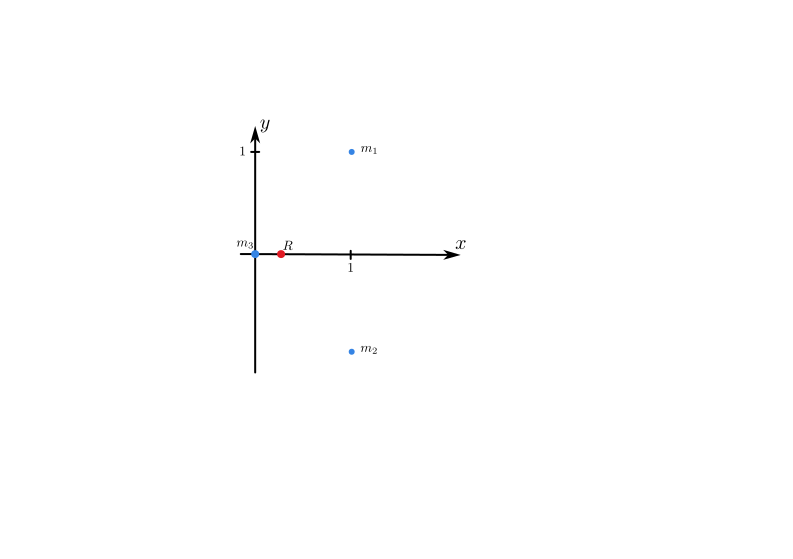
\includegraphics[width=0.3\linewidth]{../images/fig3_15.png}
    \captionsetup{width=0.7\linewidth}
    \caption{Three particles of mass $m_1$, $m_2$ and $m_3$ at positions $\vb{r}_1$,
    $\vb{r}_2$, and $\vb{r}_3$ respectively. The center of mass is at $R$ which is close to the 
    larger mass $m_3$.}
    \label{fig:3_15}
\end{figure}

\paragraph{3.17}
The masses of the earth and moon are approximately
\begin{align*}
    M_e \approx \qty{6.0e24}{\kg} \qand M_m \approx \qty{7.4e22}{\kg}
\end{align*}
where the distance between the center to center is $r = \num{3.8e5}$ km. Treating the center of the
earth as the origin, The position of the CM is
\begin{align*}
    R &= \frac{1}{M_e + M_m} (M_e \vb{r}_e + M_m \vb{r}_m) \\
    &= \frac{M_m}{M_e + M_m} r \\
    &= \qty{4600}{\km}
\end{align*}
Compared to the radius of the earth, $R_e = \qty{6400}{\km}$, the CM is located inside the earth.

\paragraph{3.19}
(a) The trajectory is still a parabola if the projectile exploded in midair.\\
(b) Since the CM remains at the target position $R = 100$ m, if one piece landed at $r_1 = 200$ m.
The second piece must be at $r_2 = 0$, or 100 m shy of the target position. Checking the CM
\begin{align*}
    R = \frac{1}{2m} (200 m + 0) = \qty{100}{\m}
\end{align*}
(c) If the pieces land at different times, shown by Figure \ref{fig:3_19}, the CM changes;
% fig3_19
\begin{figure}[ht]
    \centering
    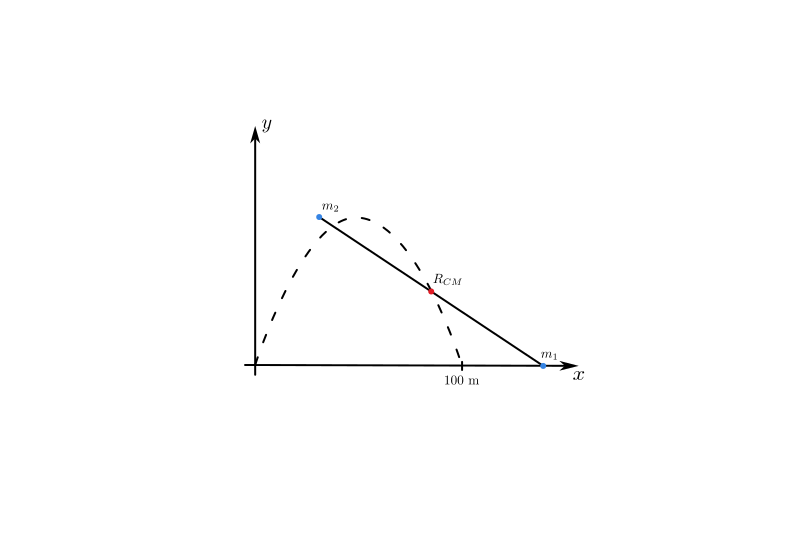
\includegraphics[width=0.4\linewidth]{../images/fig3_19.png}
    \captionsetup{width=0.7\linewidth}
    \caption{When the first piece lands on the ground, it loses all of its momentum while the second
    piece is still in projectile motion. The center of mass $R_{CM}$ will always be at the midpoint
    of the line connecting the two pieces.}
    \label{fig:3_19}
\end{figure}
The first piece that lands on the ground (beyond the target) undergoes perfect inelastic collision 
with the ground, and stops immediately. The second piece still has momentum, so the
CM will move in the direction of the second piece until it lands on the ground. Hence, the CM will
have a position $R < 100$ m.

\paragraph{3.21}
The axis of symmetry lies on the $y$-axis, so the $x$ and $z$ component of the CM is $Z = X = 0$. 
The $y$-component is given by
\begin{equation*}
    Y = \frac{1}{M} \int \sigma y \dd{A}
\end{equation*}
where $\sigma = M/A$ is the area density. Using change of variables in polar coordinates: the area
of a semicircle is $A = \pi R^2/2$ and position $y = r \sin{\theta}$. Given $\dd{A} = r \dd{r},
\dd{\theta}$ The CM position is
\begin{align*}
    Y &= \frac{2}{\pi R^2} \int_0^{\pi} \int_0^R r^2 \sin\theta \dd{r} \dd{\theta} \\
    &= \frac{2}{\pi R^2} \frac{R^3}{3} \int_0^{\pi} \sin\theta  \\
    Y & = \frac{4}{3\pi}R
\end{align*}

\paragraph{3.23}
(a) The equation of motion in vector form is $\vb{r} = \vb{v}_ot - \vb{g} t^2/2$. 
Plotting grenade trajectory with parameters $\vb{v}_o = (4,4)$, $g = 1$, from $0\le t\le 4$:
\begin{figure} [ht]
    \centering
    \includegraphics[width=0.5\linewidth]{../images/fig3_23a.png}
    \captionsetup{width=0.7\linewidth}
    \caption{The trajectory of a grenade with initial velocity $\vb{v}_o = (4,4)$ and $g = 1$.}
    \label{fig:3_23}
\end{figure}

(b) From the conservation of momentum
\begin{align*}
    P_i &= P_f \\
    2m\vb{v} &= m\vb{v}_1 + m\vb{v}_2 \\
    \vb{v}_2 &= 2\vb{v} - \vb{v}_1
\end{align*}
where $\vb{v}_1 = \vb{v} + \Delta \vb{v}$, hence $\vb{v}_2 = \vb{v} - \Delta\vb{v}$. 

(c) Given $\Delta\vb{v} = (1,3)$. Python Code:
\lstinputlisting[language=python]{../code/3_23.py}
OUTPUT:
\begin{figure}[ht]
    \centering
    \includegraphics[width=0.5\linewidth]{../images/fig3_23b.png}
    \captionsetup{width=0.8\linewidth}
    \caption{$R_o$ is the trajectory of a grenade from time $t = [0,4]$ before the explosion. After
    the grenade explodes, the two pieces follow the trajectories $R_1$ and $R_2$. The position is
    marked at $t = \numlist{0;1;2;3;4;5;6;7;8;9}$ s.}
    \label{fig:3_23c}
\end{figure}

Since the two pieces have the same mass, the CM is at the midpoint of the line connecting the two
pieces as shown in Figure \ref{fig:3_23c}. This follows the initial parabolic trajectory of the
grenade before the explosion.

\paragraph{3.25}
From the conservation of angular momentum
\begin{align*}
    l_o &= l_f \\
    m r_o^2 \omega_o &= m r^2 \omega \\
    \omega &= \frac{r_o^2}{r^2} \omega_o
\end{align*}

\paragraph{3.27}
The planets position in polar coordinates:
\begin{align*}
    \vb{r} = r\cos\theta \vu{x} + r\sin\theta \vu{y} = r \vu{r}
\end{align*}
(a) Given $\vb{\dot{r}} = \dot{r} \vu{r} + r \dot{\phi} \vu*{\phi}$, the angular momentum is
\begin{align*}
    \vb*{\ell} &= \vb{r} \cross \vb{p} \\
    &= m \vb{r} \cross \vb{\dot{r}} \\
    &= mr \vu{r} \cross (\dot{r} \vu{r} + r \dot{\phi} \vu*{\phi}) \\
    &= mr^2 \vu{r} \cp \vu*{\phi} \\
    \vb*{\ell} &= m r^2 \dot{\phi} \vu{z} 
\end{align*}
where $\dot \phi = \omega$, the angular velocity. Hence, the magnitude is $\ell = mr^2 \omega$.

(b) The change in area of the orbiting planet is given by the area of the triangle of base $r$ and
height $r\Delta \phi = r(\phi(t+\Delta t) - \phi(t))$ which is
\begin{align*}
    \Delta A = \frac{1}{2} r^2 \Delta \phi
\end{align*}
dividing both sides by $\Delta t$ and taking the limit $\Delta t \to 0$
\begin{align*}
    \lim_{\Delta t \to 0} \frac{\Delta A}{\Delta t} 
    &= \lim_{\Delta t \to 0} \frac{1}{2} r^2 \frac{\Delta \phi}{\Delta t}
\end{align*}
which gives
\begin{align*}
    \dv{A}{t} = \frac{1}{2} r^2 \omega = \frac{\ell}{2m}
\end{align*}
The rate of change of area is constant, hence the swept areas are equal for equal changes in times.

\paragraph{3.29}
Given the initial angular momentum of the spherical asteroid to be
\begin{equation*}
    \ell_o = \frac{2}{5} M_o R_o^2 \omega_o
\end{equation*}
where $M = \rho V$ and the volume of the sphere $V = 4/3 \pi R^3$. When $R = 2R_o$, the angular
momentum is conserved:
\begin{align*}
    \frac{2}{5} M R^2 \omega &= \frac{2}{5} M_o R_o^2 \omega_o \\
    \omega &= \frac{V_o}{4V} \omega_o \\
    \omega &= \frac{1}{32} \omega_o
\end{align*}

\paragraph{3.31}
Moment of inertia as an integral
\begin{equation*}
    I = \int r^2 \dd{m}
\end{equation*}
where $\dd{m} = \sigma \dd{A}$. The area density of a uniform disc is $\sigma = M / A$ where
$A = \pi R^2$, the area of a circle. Using polar coordinates, change of variables gives
\begin{equation*}
    \dd{A} = r \dd{r} \dd{\theta}
\end{equation*}
The moment of inertia is
\begin{align*}
    I &= \sigma \int_0^R \int_0^{2\pi} (r^2) r \dd{r} \dd{\theta} \\
    &= \sigma \int_0^R r^3 \dd{r} \int_0^{2\pi} \dd{\theta} \\
    &= \sigma \frac{R^4}{4} 2\pi \\
    I &= \frac{1}{2} M R^2
\end{align*}

\paragraph{3.33}
A uniform thin square of side $2b$ lies on the $xy$ plane and rotates about an axis through its
center and perpendicular to the square itself. The distance of the point mass from the axis is
\begin{align*}
    r = \sqrt{x^2 + y^2}
\end{align*}
where $x = y$ for a square with its center at the origin. With $dm = \sigma \dd{A}$, and area of the
square $A = (2b)^2$, the moment of inertia is
\begin{align*}
    I &= \sigma \int r^2  \dd{A} \\
    &= \sigma \int_{-b}^{b} \int_{-b}^{b} (x^2 + y^2) \dd{x} \dd{y} \\
    &= \frac{8}{3} \sigma b^4 \\
    &= \frac{2}{3} M b^2
\end{align*}

\paragraph{3.35}
\begin{figure}[ht]
    \centering
    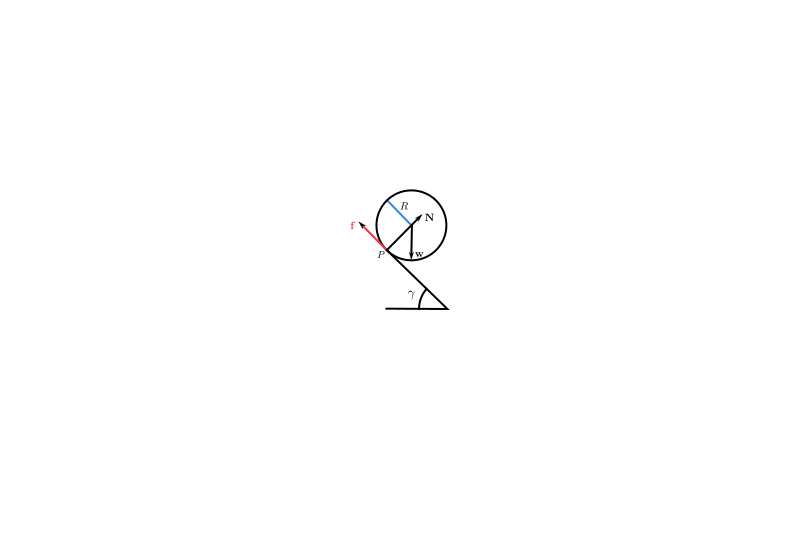
\includegraphics[width=0.3\linewidth]{../images/fig3_35.png}
    \captionsetup{width=0.7\linewidth}
    \caption{A uniform solid disk of mass $M$ and radius $R$ is rolling without slipping down an
    incline at an angle $\gamma$ to the horizontal. The point of contact between the disk and
    incline is at $P$. The forces acting on the point of contact are the normal force $\vb{N}$, the 
    weight $\vb{w}$ and the frictional force $\vb{f}$.}
    \label{fig:3_35}
\end{figure}
(a) The free-body diagram of the disk is shown in Figure \ref{fig:3_35}.

(b) Given the moment of inertia about point $P$ is $I_P = \frac{3}{2} MR^2$ and the external torque
$\Gamma^{ext} = R Mg \sin{\gamma}$. From conservation of anuglar momentum
\begin{align*}
    \dot{L} &= \Gamma^{ext} \\
    I_p \dot \omega &= RMg \sin{\gamma} \\
    \frac{3}{2} MR^2 \dot \omega &= RMg \sin{\gamma} \\
    R \dot \omega &= \frac{2}{3} g\sin{\gamma}
\end{align*}
where $R\dot{\omega} = \dot{v}$ is the angular acceleration.

(c) Applying $\dot{L} = \Gamma^{ext}$ to the rotation about the CM: Finding the frictional force
from Newton's Second law only requires the component parallel to the incline
\begin{align*}
    f = Mg \sin{\gamma} - M\dot{v}
\end{align*}
The torque about the CM is $\Gamma^{ext} = fR$. The angular acceleration is
\begin{align*}
    fR &= I_{CM} \dot{\omega} \\
    MgR\sin{\gamma} - MR\dot{v} &= \frac{1}{2} MR^2 \dot{\omega} \\
    gR \sin{\gamma} &= \frac{1}{2} R \dot{v} + \dot{v} \\
    \dot{v} &= \frac{2}{3} g \sin{\gamma}
\end{align*}

\paragraph{3.37}
\begin{figure}[ht]
    \centering
    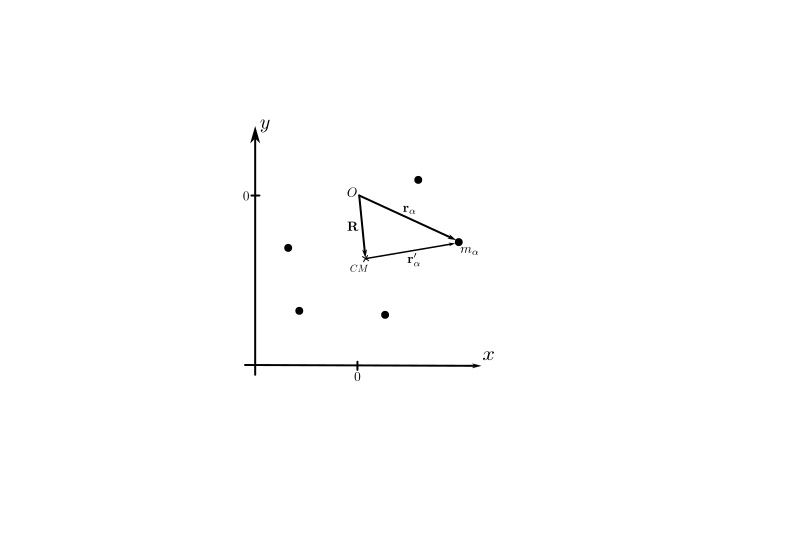
\includegraphics[width=0.3\linewidth]{../images/fig3_37.png}
    \captionsetup{width=0.7\linewidth}
    \caption{A system of $N$ particles of masses $m_{\alpha}$ at positions $\vb{r}_{\alpha}$ 
    relative to origin $O$. The center of mass is at $\vb{R}$ and the position of $m_{\alpha}$
    relative to the CM is $\vb{r}_{\alpha}'$.}
    \label{fig:3_37}
\end{figure}
(a) From Figure \ref{fig:3_37}, the position of the center of mass is
\begin{equation*}
    \vb{r}_{\alpha}' = \vb{r}_{\alpha} - \vb{R}
\end{equation*}

(b) Given $\sum \vb{r}_{\alpha} = \vb{R}$ and the mass of the system $M = \sum m_{\alpha}$:
\begin{align*}
    \sum m_{\alpha} \vb{r}_{\alpha}' &= \sum m_{\alpha} (\vb{r}_{\alpha} - \vb{R}) \\
    &= \sum m_{\alpha} \vb{r}_{\alpha} - \sum m_{\alpha} \vb{R} \\
    &= M \vb{R} - M \vb{R} \\
    &= 0
\end{align*}
Obviously, the CM is at the origin if the \textit{frame of reference} is at the CM.

(c) The angular momentum about the CM is
\begin{align*}
    \vb{L} = \sum \vb{r}_{\alpha}' \cp \vb{p}_{\alpha}'
    = \sum m_{\alpha} \vb{r}_{\alpha}' \cp \dot{\vb{r}}_{\alpha}'
\end{align*}
taking the time derivative
\begin{align*}
    \dot{\vb{L}} &= \sum m_{\alpha} \dot{\vb{r}}_{\alpha}' \cp \dot{\vb{r}}_{\alpha}'
        + \sum m_{\alpha} \vb{r}_{\alpha}' \cp \ddot{\vb{r}}_{\alpha}' \\
    &= \sum m_{\alpha} \vb{r}_{\alpha}' \cp \ddot{\vb{r}}_{\alpha}' \\
    &= \sum m_{\alpha} \vb{r}_{\alpha}' \cp (\ddot{\vb{r}}_{\alpha} - \ddot{\vb{R}}) \\
    &= \sum  \vb{r}_{\alpha}' \cp m_{\alpha} \ddot{\vb{r}}_{\alpha} 
        - \ddot{\vb{R}} \sum m_{\alpha} \vb{r}_{\alpha}' \\
    &= \sum \vb{r}_{\alpha}' \cp \vb{F}_{\alpha}^{ext} \\
    &= \vb{\Gamma}^{ext}
\end{align*}
where the internal forces cancel out from Newton's third law. Hence, the angular momentum about
the CM is equal to the external torque.
\end{document}